\documentclass{standalone}
%-----------------------------------------------------------------------------%
%%% Color %%%
\usepackage{xcolor}
\definecolor{myred}{RGB}{229,0,0}
\definecolor{myblue}{RGB}{0,98,144}
\definecolor{myyellow}{RGB}{246,182,50}
\newcommand{\red}[1]{\textcolor{myred}{#1}}
\newcommand{\blue}[1]{\textcolor{myblue}{#1}}
\newcommand{\yellow}[1]{\textcolor{myyellow}{#1}}
%-----------------------------------------------------------------------------%
%%% TikZ %%%
\usepackage{tikz}
% \usetikzlibrary{calc}
% \usetikzlibrary{positioning}
% \usetikzlibrary{patterns}
% \usetikzlibrary{fit}
% \usetikzlibrary{angles,quotes}
% \usetikzlibrary{intersections}
% \usetikzlibrary{decorations.markings}
%-----------------------------------------------------------------------------%

\begin{document}

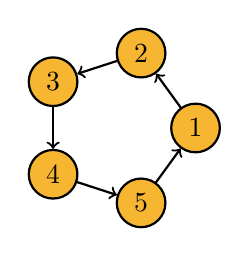
\begin{tikzpicture}[thick,line cap=round]
	\tikzstyle{bai}=[solid,circle,draw,inner sep=.8pt,fill=white];
	\tikzstyle{hei}=[solid,circle,draw,inner sep=.8pt,fill];
	% \node[bai] at (0,0) {};
	\node[draw,circle,fill=myyellow] (1) at (000:1) {$1$};
	\node[draw,circle,fill=myyellow] (2) at (072:1) {$2$};
	\node[draw,circle,fill=myyellow] (3) at (144:1) {$3$};
	\node[draw,circle,fill=myyellow] (4) at (216:1) {$4$};
	\node[draw,circle,fill=myyellow] (5) at (288:1) {$5$};
	\draw[->] (1) to (2);
	\draw[->] (2) to (3);
	\draw[->] (3) to (4);
	\draw[->] (4) to (5);
	\draw[->] (5) to (1);
\end{tikzpicture}

\end{document}
